\chapter{Tunable Laser with on Chip Controllable Feedback}\label{ch:laser_with_on_chip_feedback}
\section{Design}\label{sec:design}
The design of the on chip controllable feedback is targeting to the region I (phase dependent linewidth reduction) and region V (strong feedback with coumpound cavity mode) in the studied five feedabck regions \cite{} by ustilization of the Bragg grating, Multimode Interferometer (MMI), Variable Optical Attenuator (VOA) and Thin Film Filter (TFF) structures on our Polyboard platform. 
% \begin{figure}[ht]
%     \centering
%     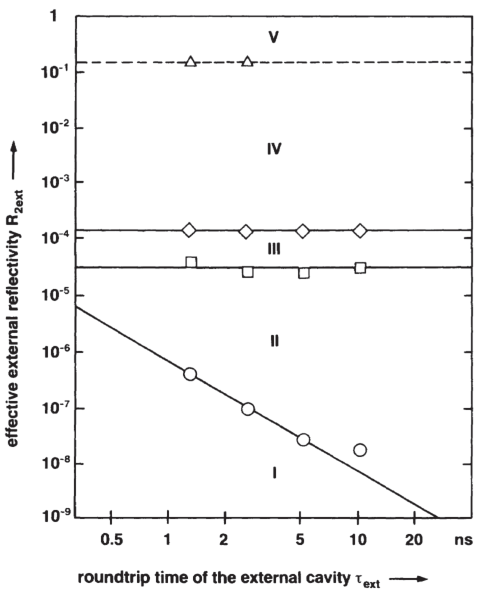
\includegraphics[width=10cm]{figures/feedback_region.PNG}
%     \caption{Feedback regimes for a laser diode.}
%     \label{feedback_region}
% \end{figure}


\subsection{Active and Passive Elements}
% As a variable optical attenuator (VOA) a 1x1 thermally tunable Multimode interferometer (MMI) is used (Fig.3.4.c). MMI is a multimode waveguide in which the light propagates in N modes. The various modes interfere with each other and produce an interference pattern in the MMI. This pattern allows at points of constructive interference to place output waveguide and thus to tap multiple outputs, each with a corresponding proportion of the total output power from an input signal. Depending on the design of the structure, the MMI can realize a different power division. On one side along the MMI is placed an electrode that allows using the thermo-optical effect. 
% We distinguish the states ON and OFF. In the OFF state, there is no heating of the electrodes and constructive interference takes place at the point where the output waveguide is. In ON-state, the interference pattern of the MMI is so affected, so that shifts through the partial change of the refractive index of the MMI, the position of constructive interference. Thus, a maximum interference point moves away from the position of the output waveguide and the output signal is tapped at reduced power (Fig.3.4.a and b). In this way a variable optical attenuation is created.
% An input waveguide with a width and height of 3.2 µm leads light into the interferometer. The height of the MMI (x-axis) also corresponds to 3.2 µm, the width is 18 µm and the length is 380 µm. The light that is leaving the MMI is received by an output waveguide. Height and width of the output waveguide coincide with the dimensions of the input waveguide. The transition of the input and output waveguide of the MMI is realized with taper sections that reduce the coupling losses. This VOA design was showing the best results compare to the literature [16-18].
The grating is designed to have its Bragg wavelength at $\lambda_B=1550 \ nm$.  Variable Optical Attenuator (VOA) is acheived with a $1\times 1$  thermally tunable MMI by placing an electrode on the side along the MMI which allows the thermo-optical effect. Thin Film Filter (TFF) acts as a high reflectivity mirror with its operating wavelength covers the grating Bragg wavelength, it can be simply inserted in the TFF slot thanks to our Polyboard technology. The characterization example of the VOA is shown in \autoref{fig:VOA_18321}. Maximum $-28.39 \ dB$ damping was achieved at current value of $54 \ mA$. 

% The Multimode Interferometer (MMI) is a multimode waveguide in which the light propagates in N modes. The various modes interfere with each other and produce an interference pattern in the MMI. This pattern allows at points of constructive interference to place output waveguide and thus to tap multiple outputs, each with a corresponding proportion of the total output power from an input signal. Depending on the design of the structure, the MMI can realize a different power division.

\begin{figure}[ht]
    \centering
    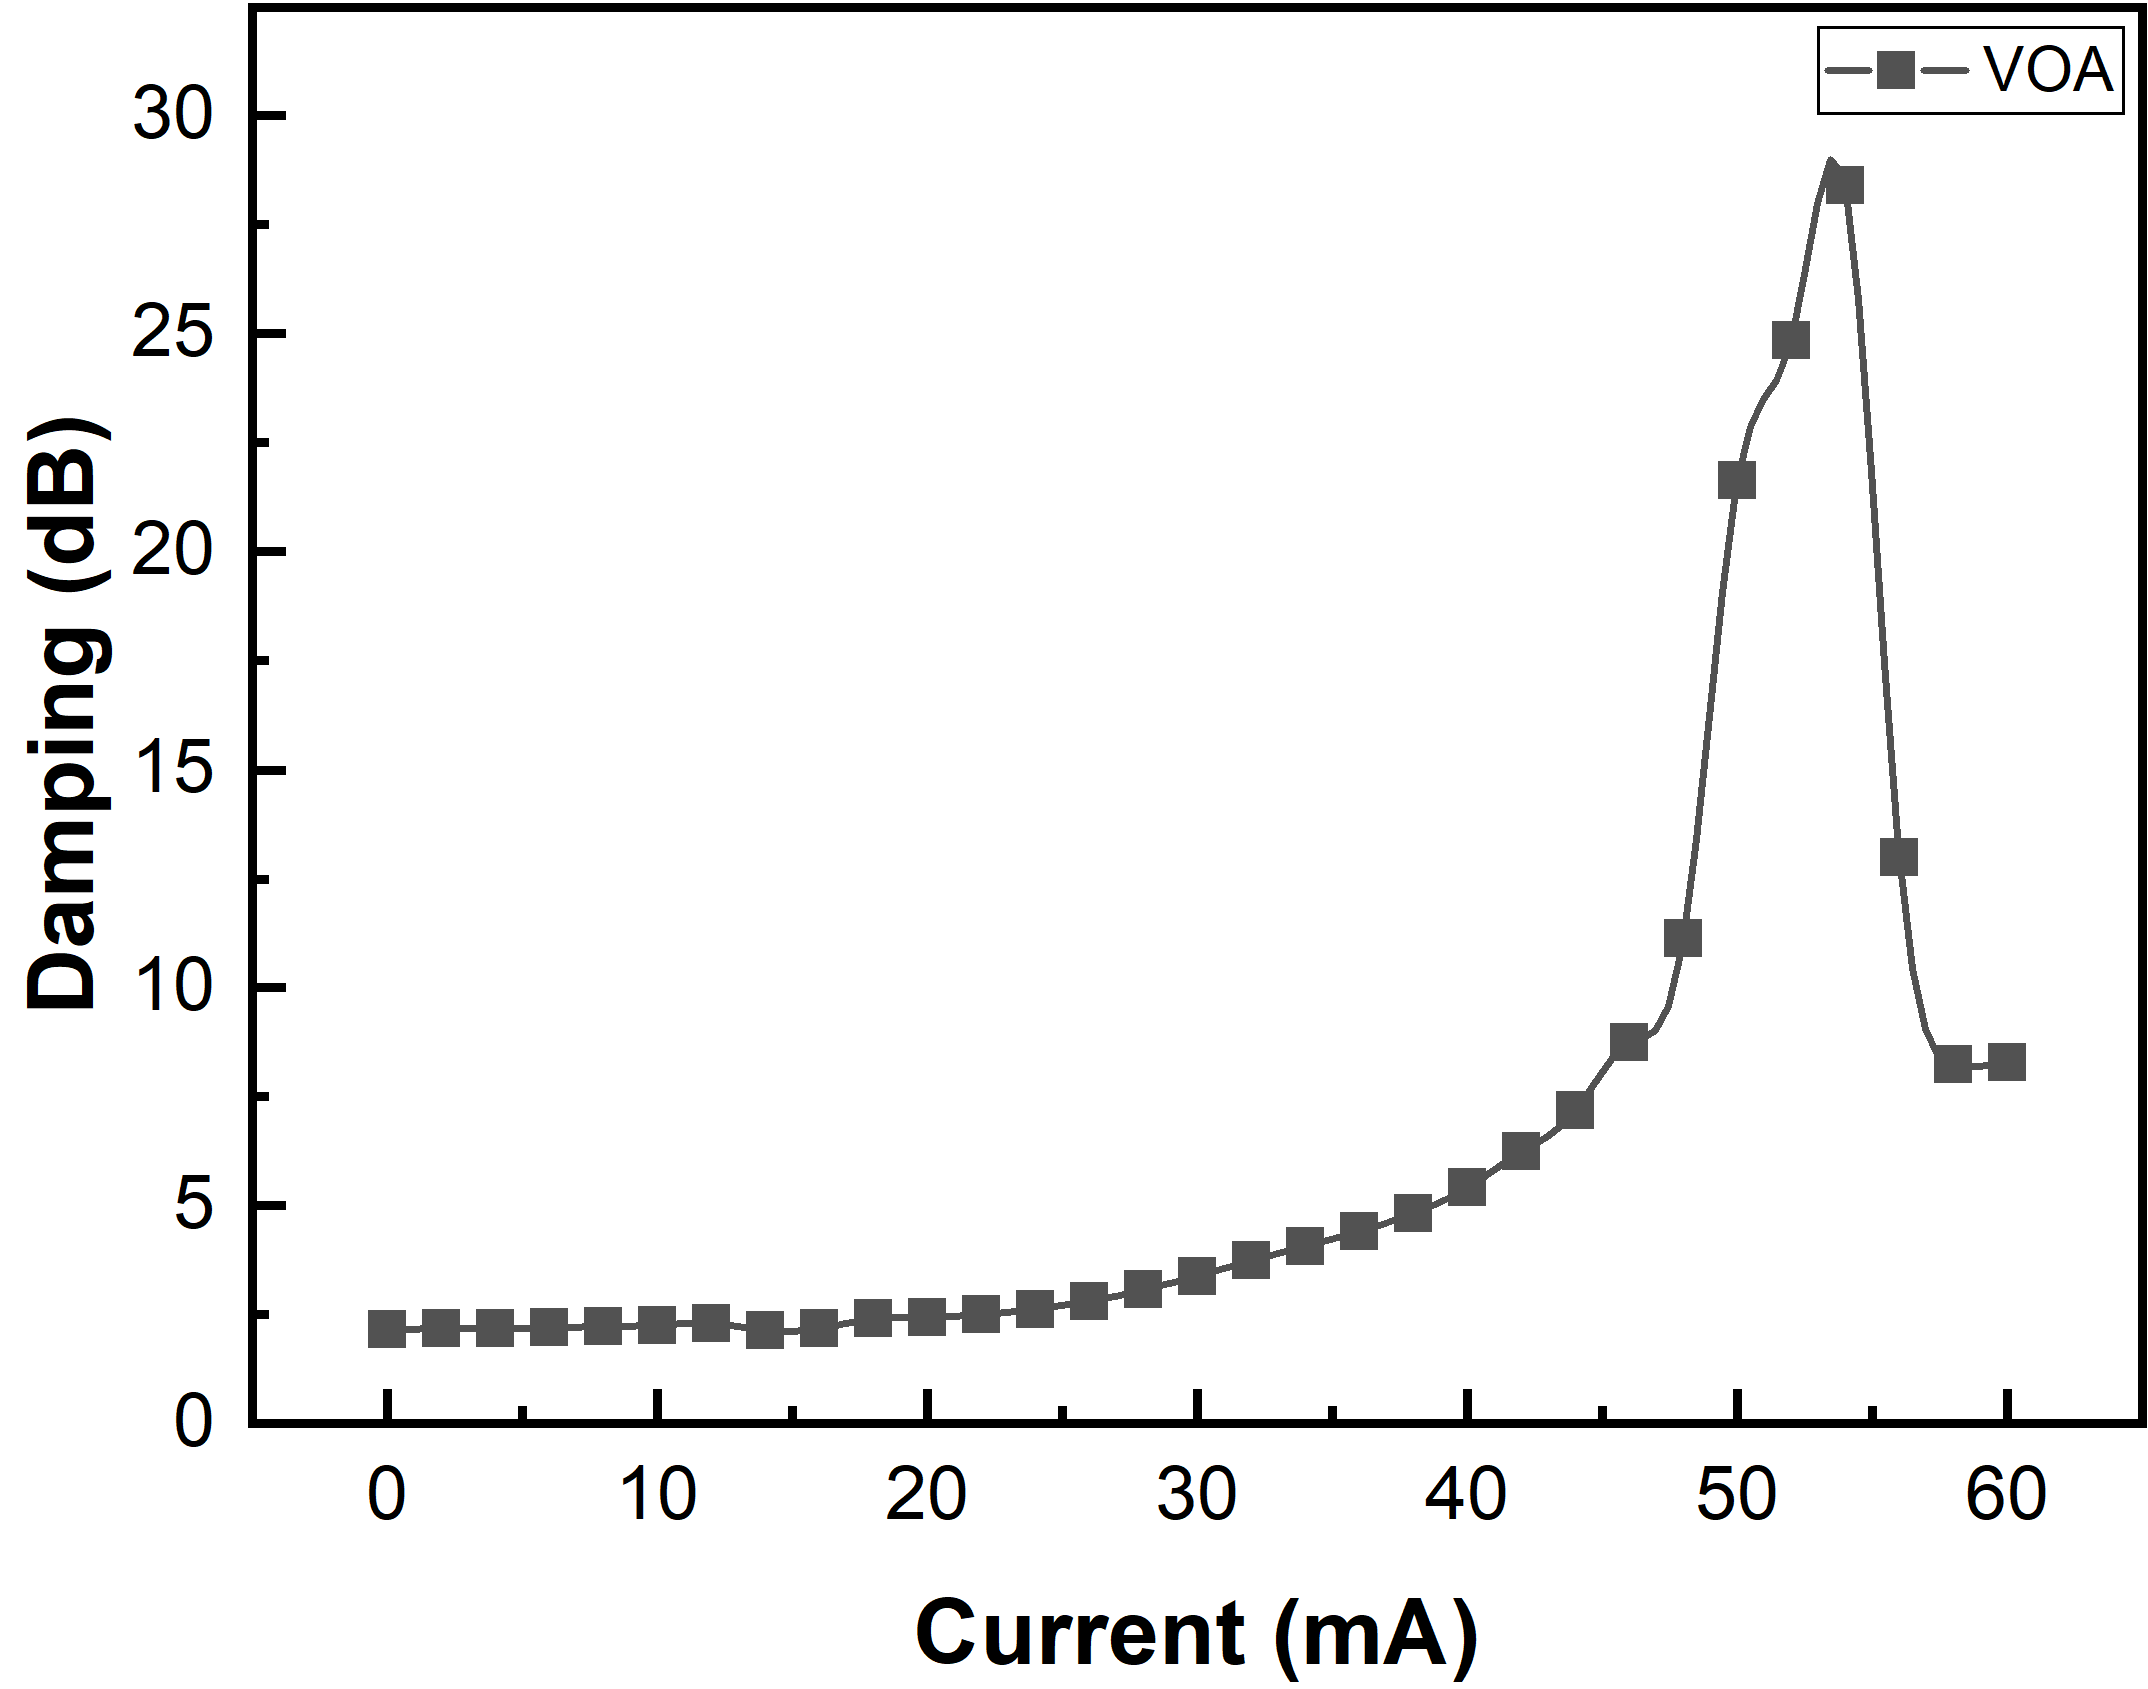
\includegraphics[width=0.55\linewidth]{figures/VOA_18321.png}
    \caption{Characterization of the VOA with maximum $-28.39 \ dB$ damping achieved at current value of $54 \ mA$.}
    \label{fig:VOA_18321}
\end{figure}

\subsection{Long Feedback Cavity} \label{subsec:long_feedback_cavity}
The on-chip long feedback cavity design is achieved by the spiral structure with the bending radius of $1500 \ \mu m$. The beginning of the chip is our normal tunable laser, followed by a $1\times 2$ MMI to seperate the output port and the external cavity. In the external cavity, two VOA structures and a phase section is included. The spiral structure has a variable design to achieve external cavity length of [39.28, 55.70, 81.33, 86.53, 100.75, 157.35] $\ mm$. By using \autoref{eq:F_weak_feedback} and \autoref{eq:F_strong_feedback} 
The chip design and the example of grating characterization is shown in \autoref{fig:grating_5742}. The appearing of the ripples in the reflection curves indicates the existing of the reflection besides the grating. We checked the spacing of the ripple is corresponding to the distance between the MMI and the output port. Ripples in transmission curves were not observed may because the attenuation inside the polymer waveguide after the spiral structure is relative high so that the reflected from the TFF slot got attenuated.
% \begin{figure}[!htb]
%     \centering
%     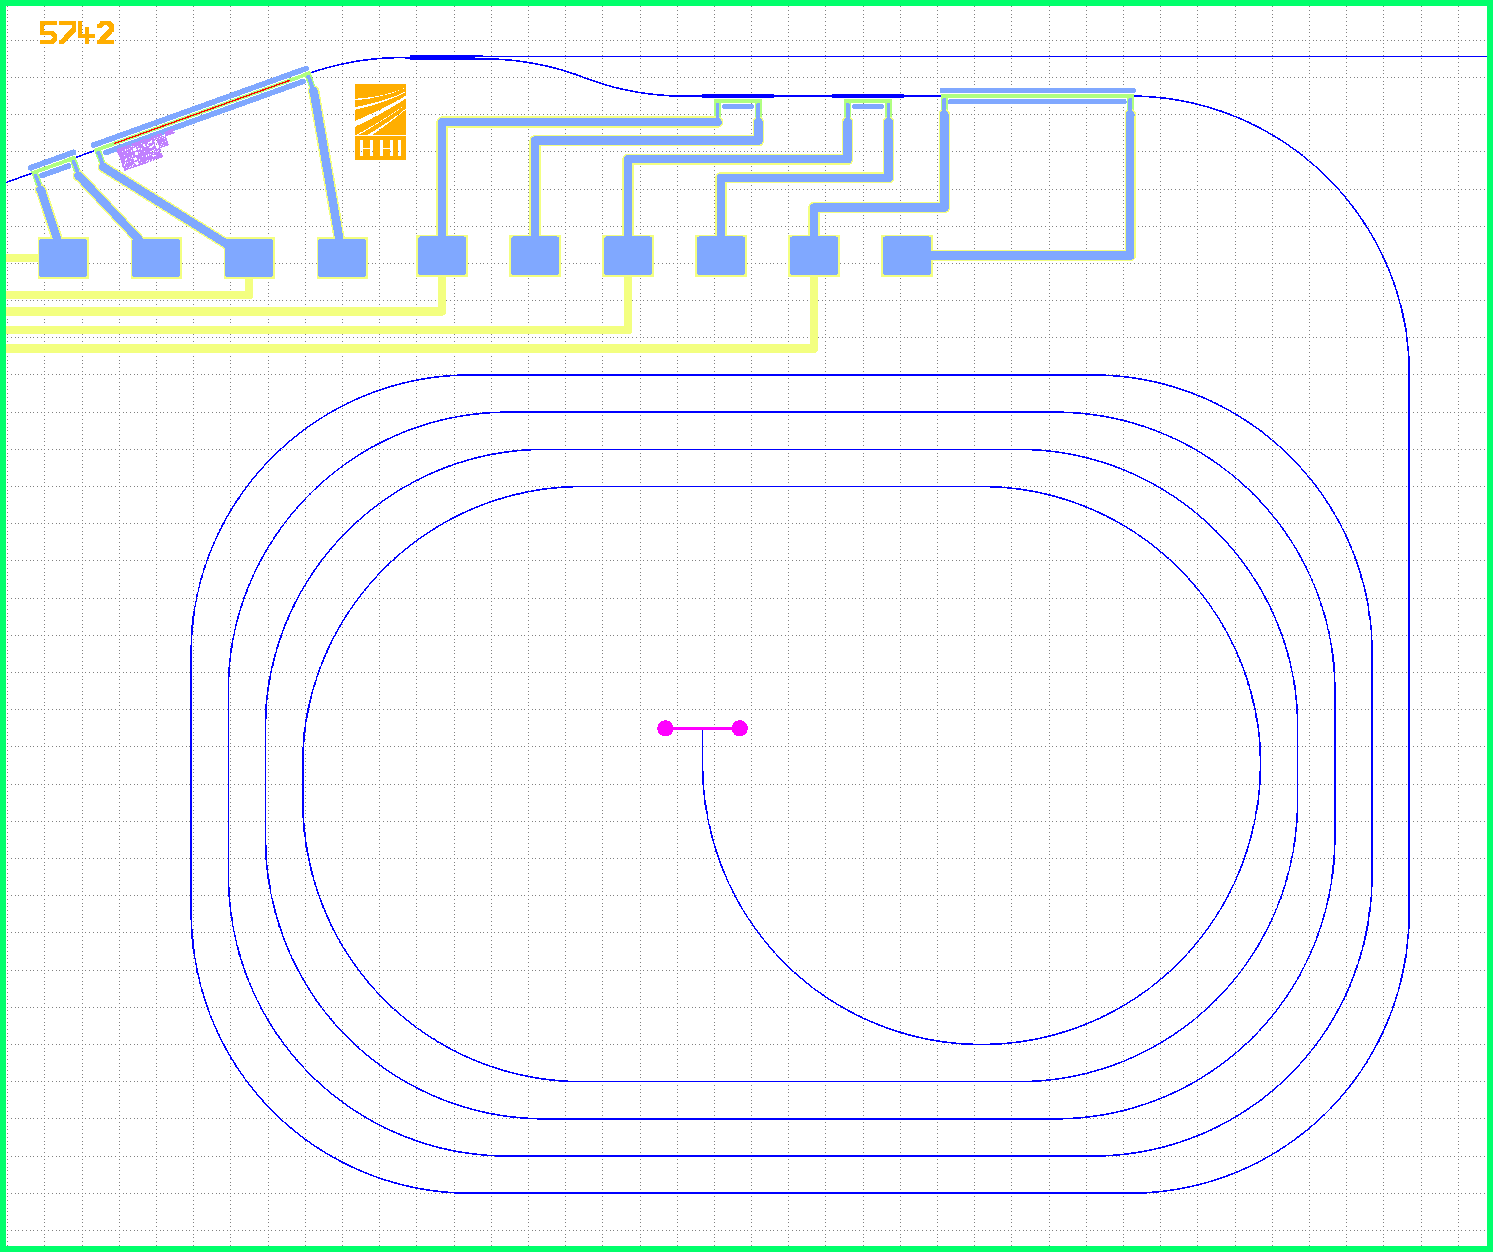
\includegraphics[width=0.6\linewidth]{figures/5742_spiral.png}
%     \caption{}
%     \label{fig:5742_spiral}
% \end{figure}

\begin{figure}[htb]
    \centering
    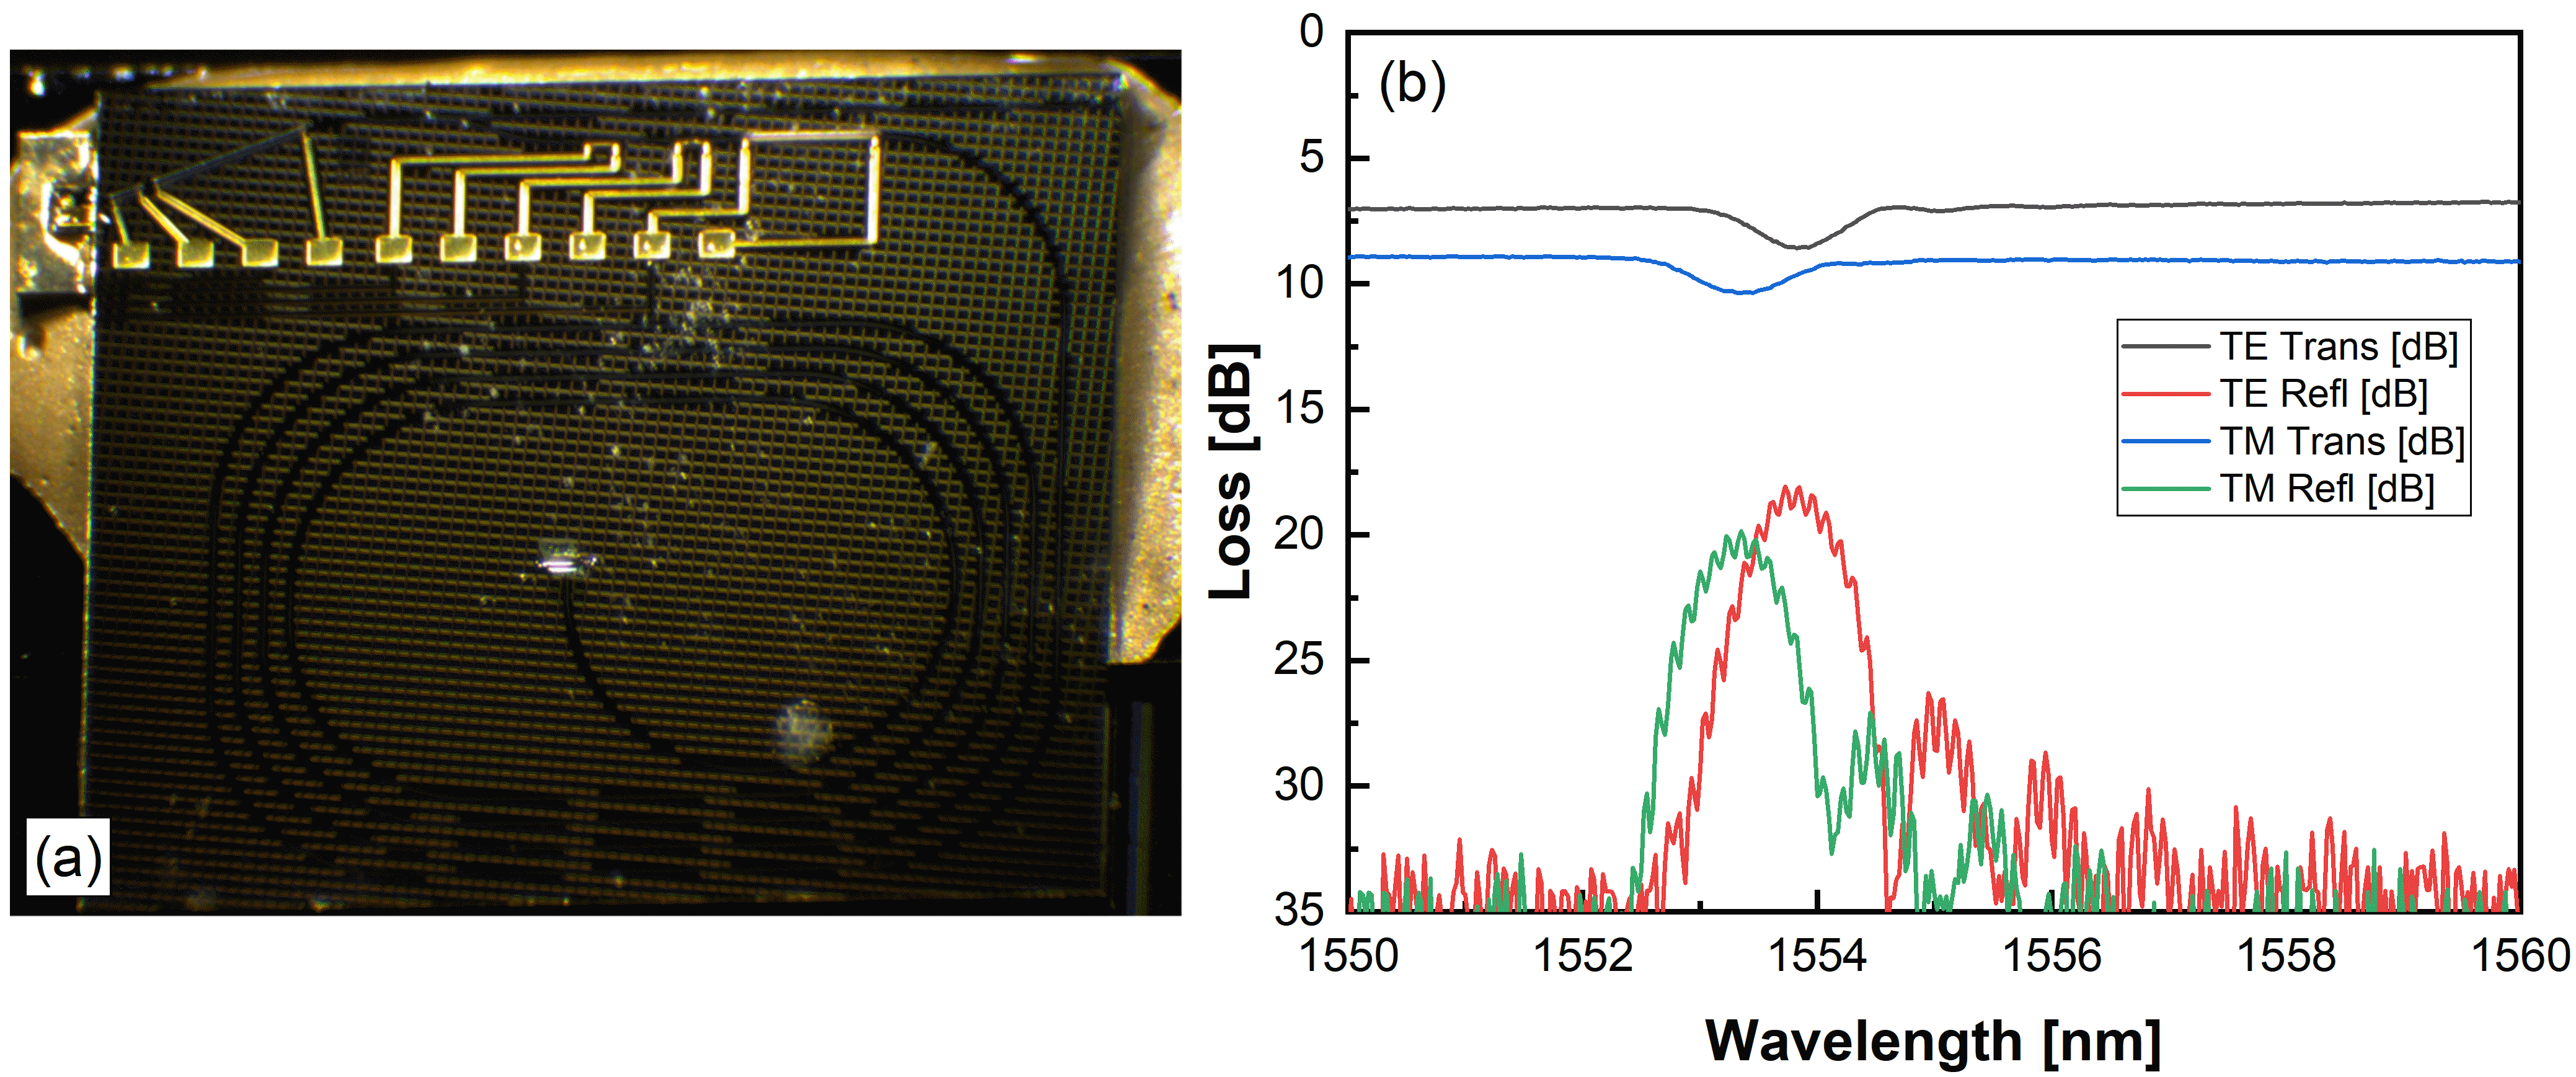
\includegraphics[width=\linewidth]{figures/grating_5742.png}
    \caption{(a) Chip design of the laser with long external cavity controllable feedback, (b) Grating characterization of the device, the spacing of the ripples in the reflection (red and green) curves are corresponding to the distance between MMI and output port.}
    \label{fig:grating_5742}
\end{figure}

\subsection{Short Feedback Cavity} \label{subsec:short_feedback_cavity}
The on-chip short feedback cavity follows the same design principle as in \autoref{subsec:long_feedback_cavity}, the chip design and the example of grating characterization is shown in \autoref{fig:grating_6559}. In order to exploit PPR, \autoref{eq:mode_spacing} is used to set the ideal cavity length. External cavity length of [3129.76, 3589,76, 3859.76, 4159.76, 4869.76, 5309.76, 6359.76] $\mu m$ are choosen according to the FSR plot shown in \autoref{fig:design_FSR}. Besides the similliar ripples in the reflection curves as in \autoref{fig:grating_5742}, reflection is also observed in the transmission curves, with the spacing corresponding to the external cavity, which indicates the reflection from the TFF slot is relatively high in this case.

\begin{figure}[ht]
    \centering
    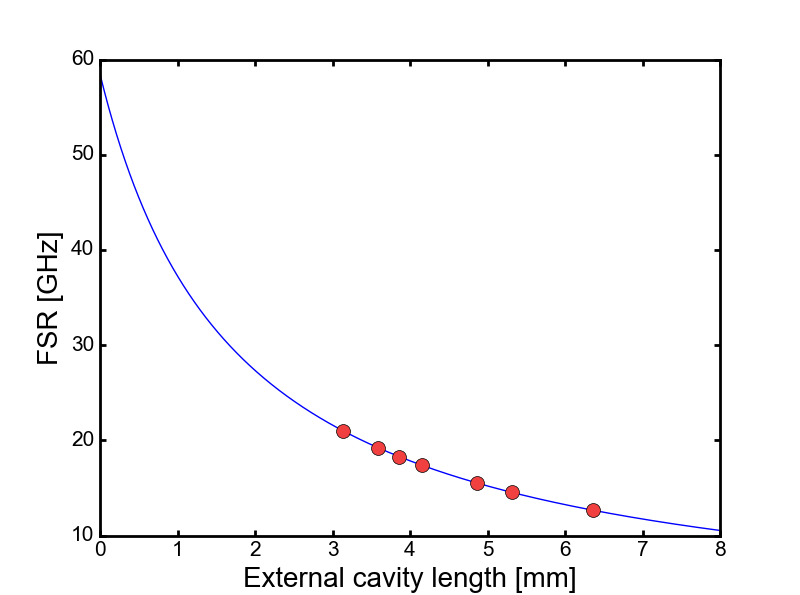
\includegraphics[width=.6\linewidth]{figures/design_FSR.png}
    \caption{FSR versus different external cavity length, the red circle markers are corresponding to the FSR of [22, 20, 19, 18, 16, 15, 13] $GHz$.}
    \label{fig:design_FSR}
\end{figure}

\begin{figure}[ht]
    \centering
    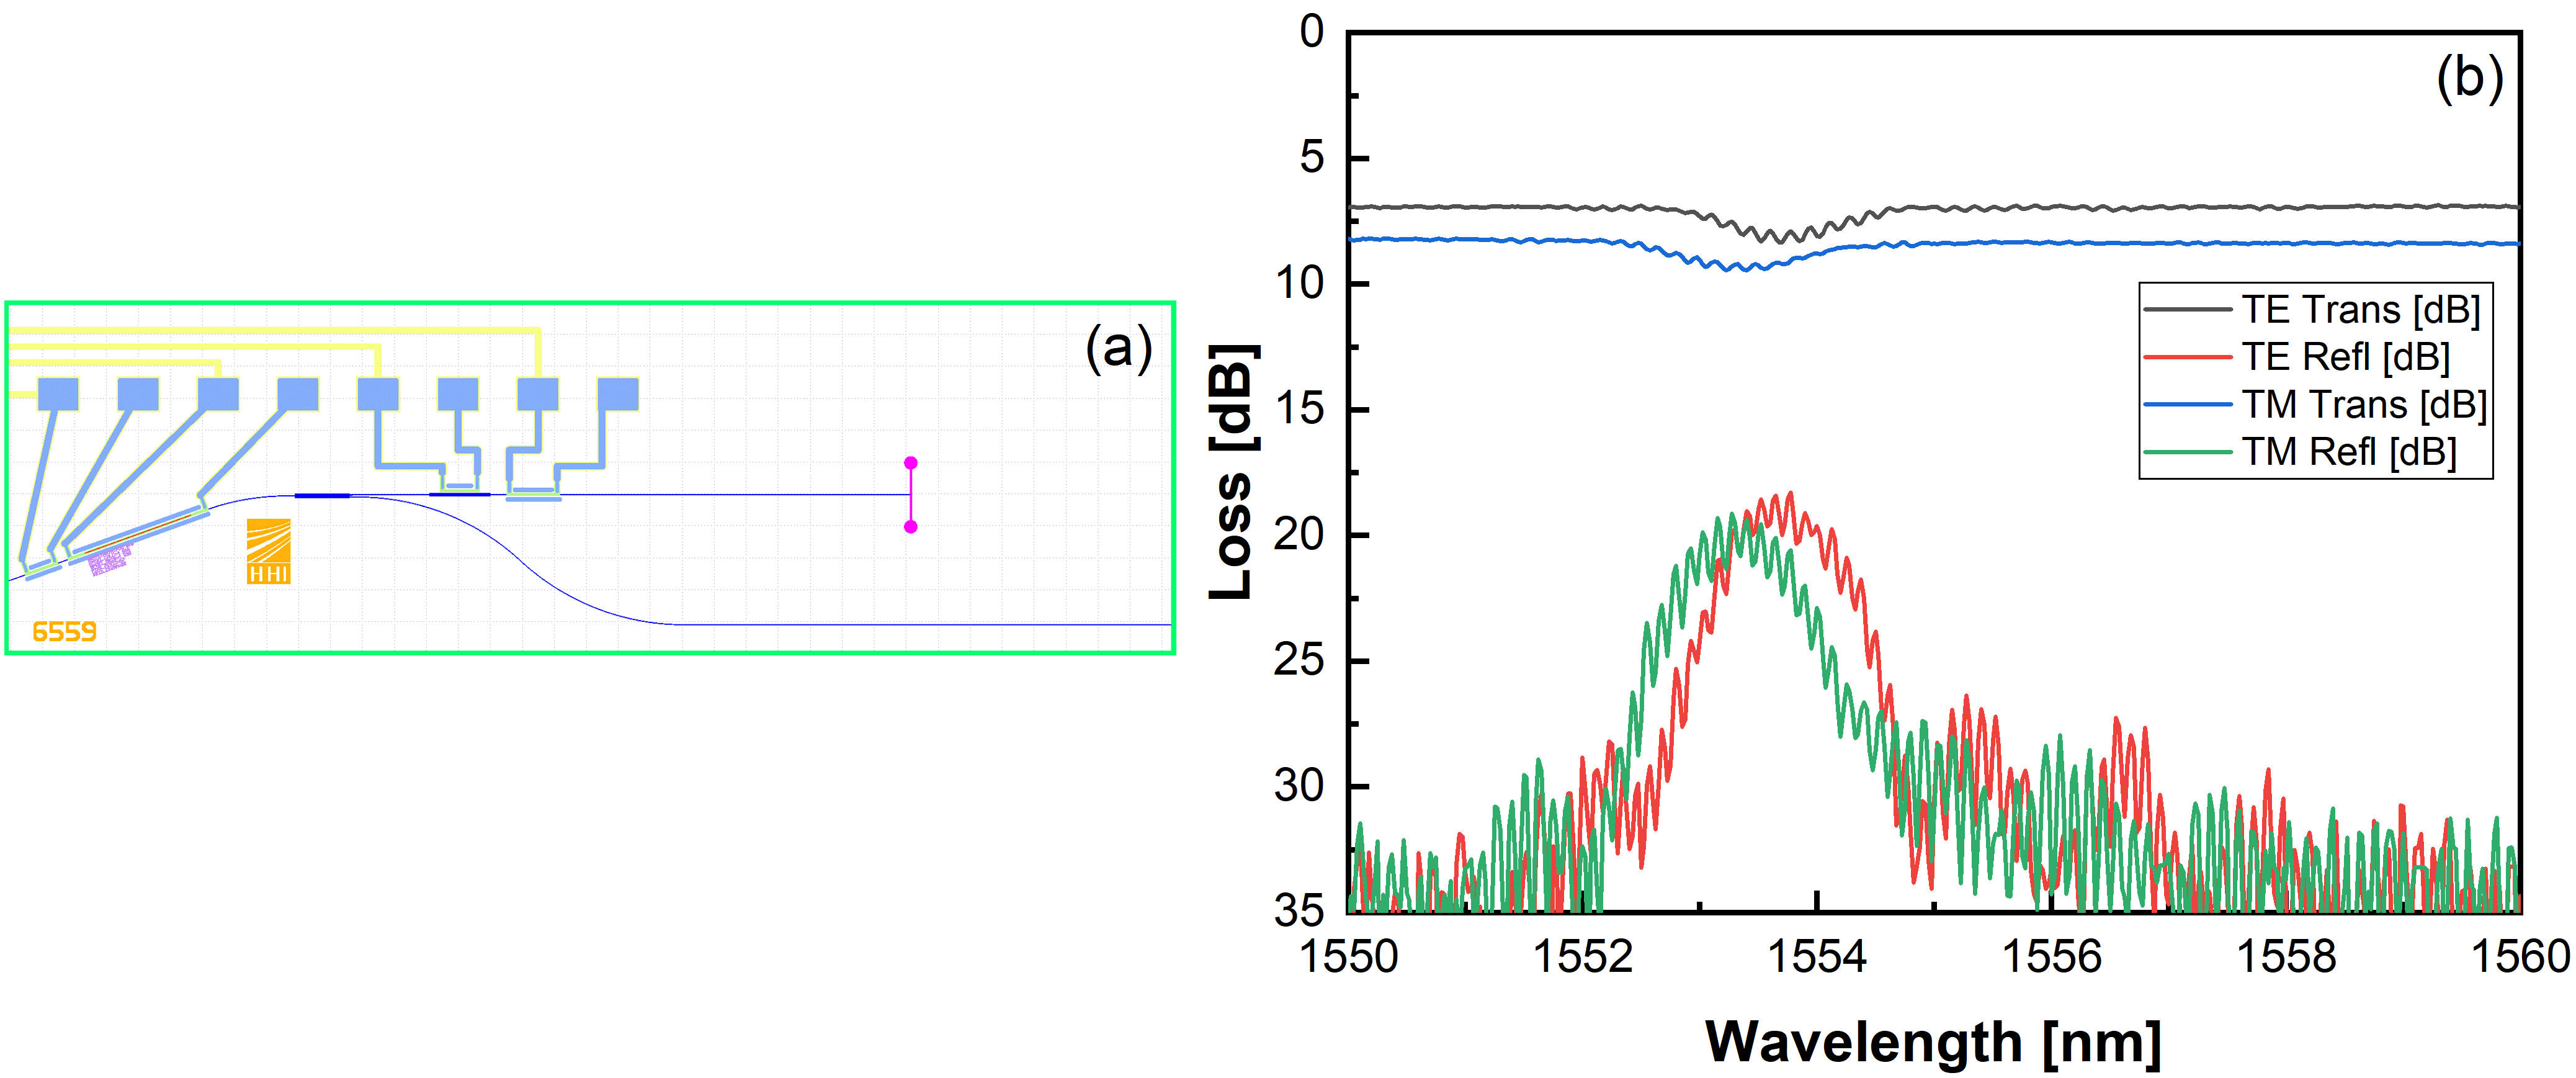
\includegraphics[width=\linewidth]{figures/grating_6559.png}
    \caption{(a) Chip design of the laser with short external cavity controllable feedback, (b) grating characterization of the device, the spacing of the ripples in the transmission (black and blue) and reflection (red and green) curves are corresponding to the length of the external cavity and the distance between MMI and output port respectively.}
    \label{fig:grating_6559}
\end{figure}


\section{Characterization}

% The parameter $F$ strongly depends on the phase of the externally reflected light $\phi_{ext}$ a very careful control of $\phi_{ext}$ is required for achieving a certain linewidth narrowing

Bandwidth enhancement by PPR is achieved with the short external cavity design. As shown in \autoref{fig:spectra_and_bandwidth_6559}, the appearing of the second resonance peak in the frequency response is clearly different from the ones we achieved in \autoref{fig:undamped_RO}.

\begin{figure}[!htb]
    \centering
    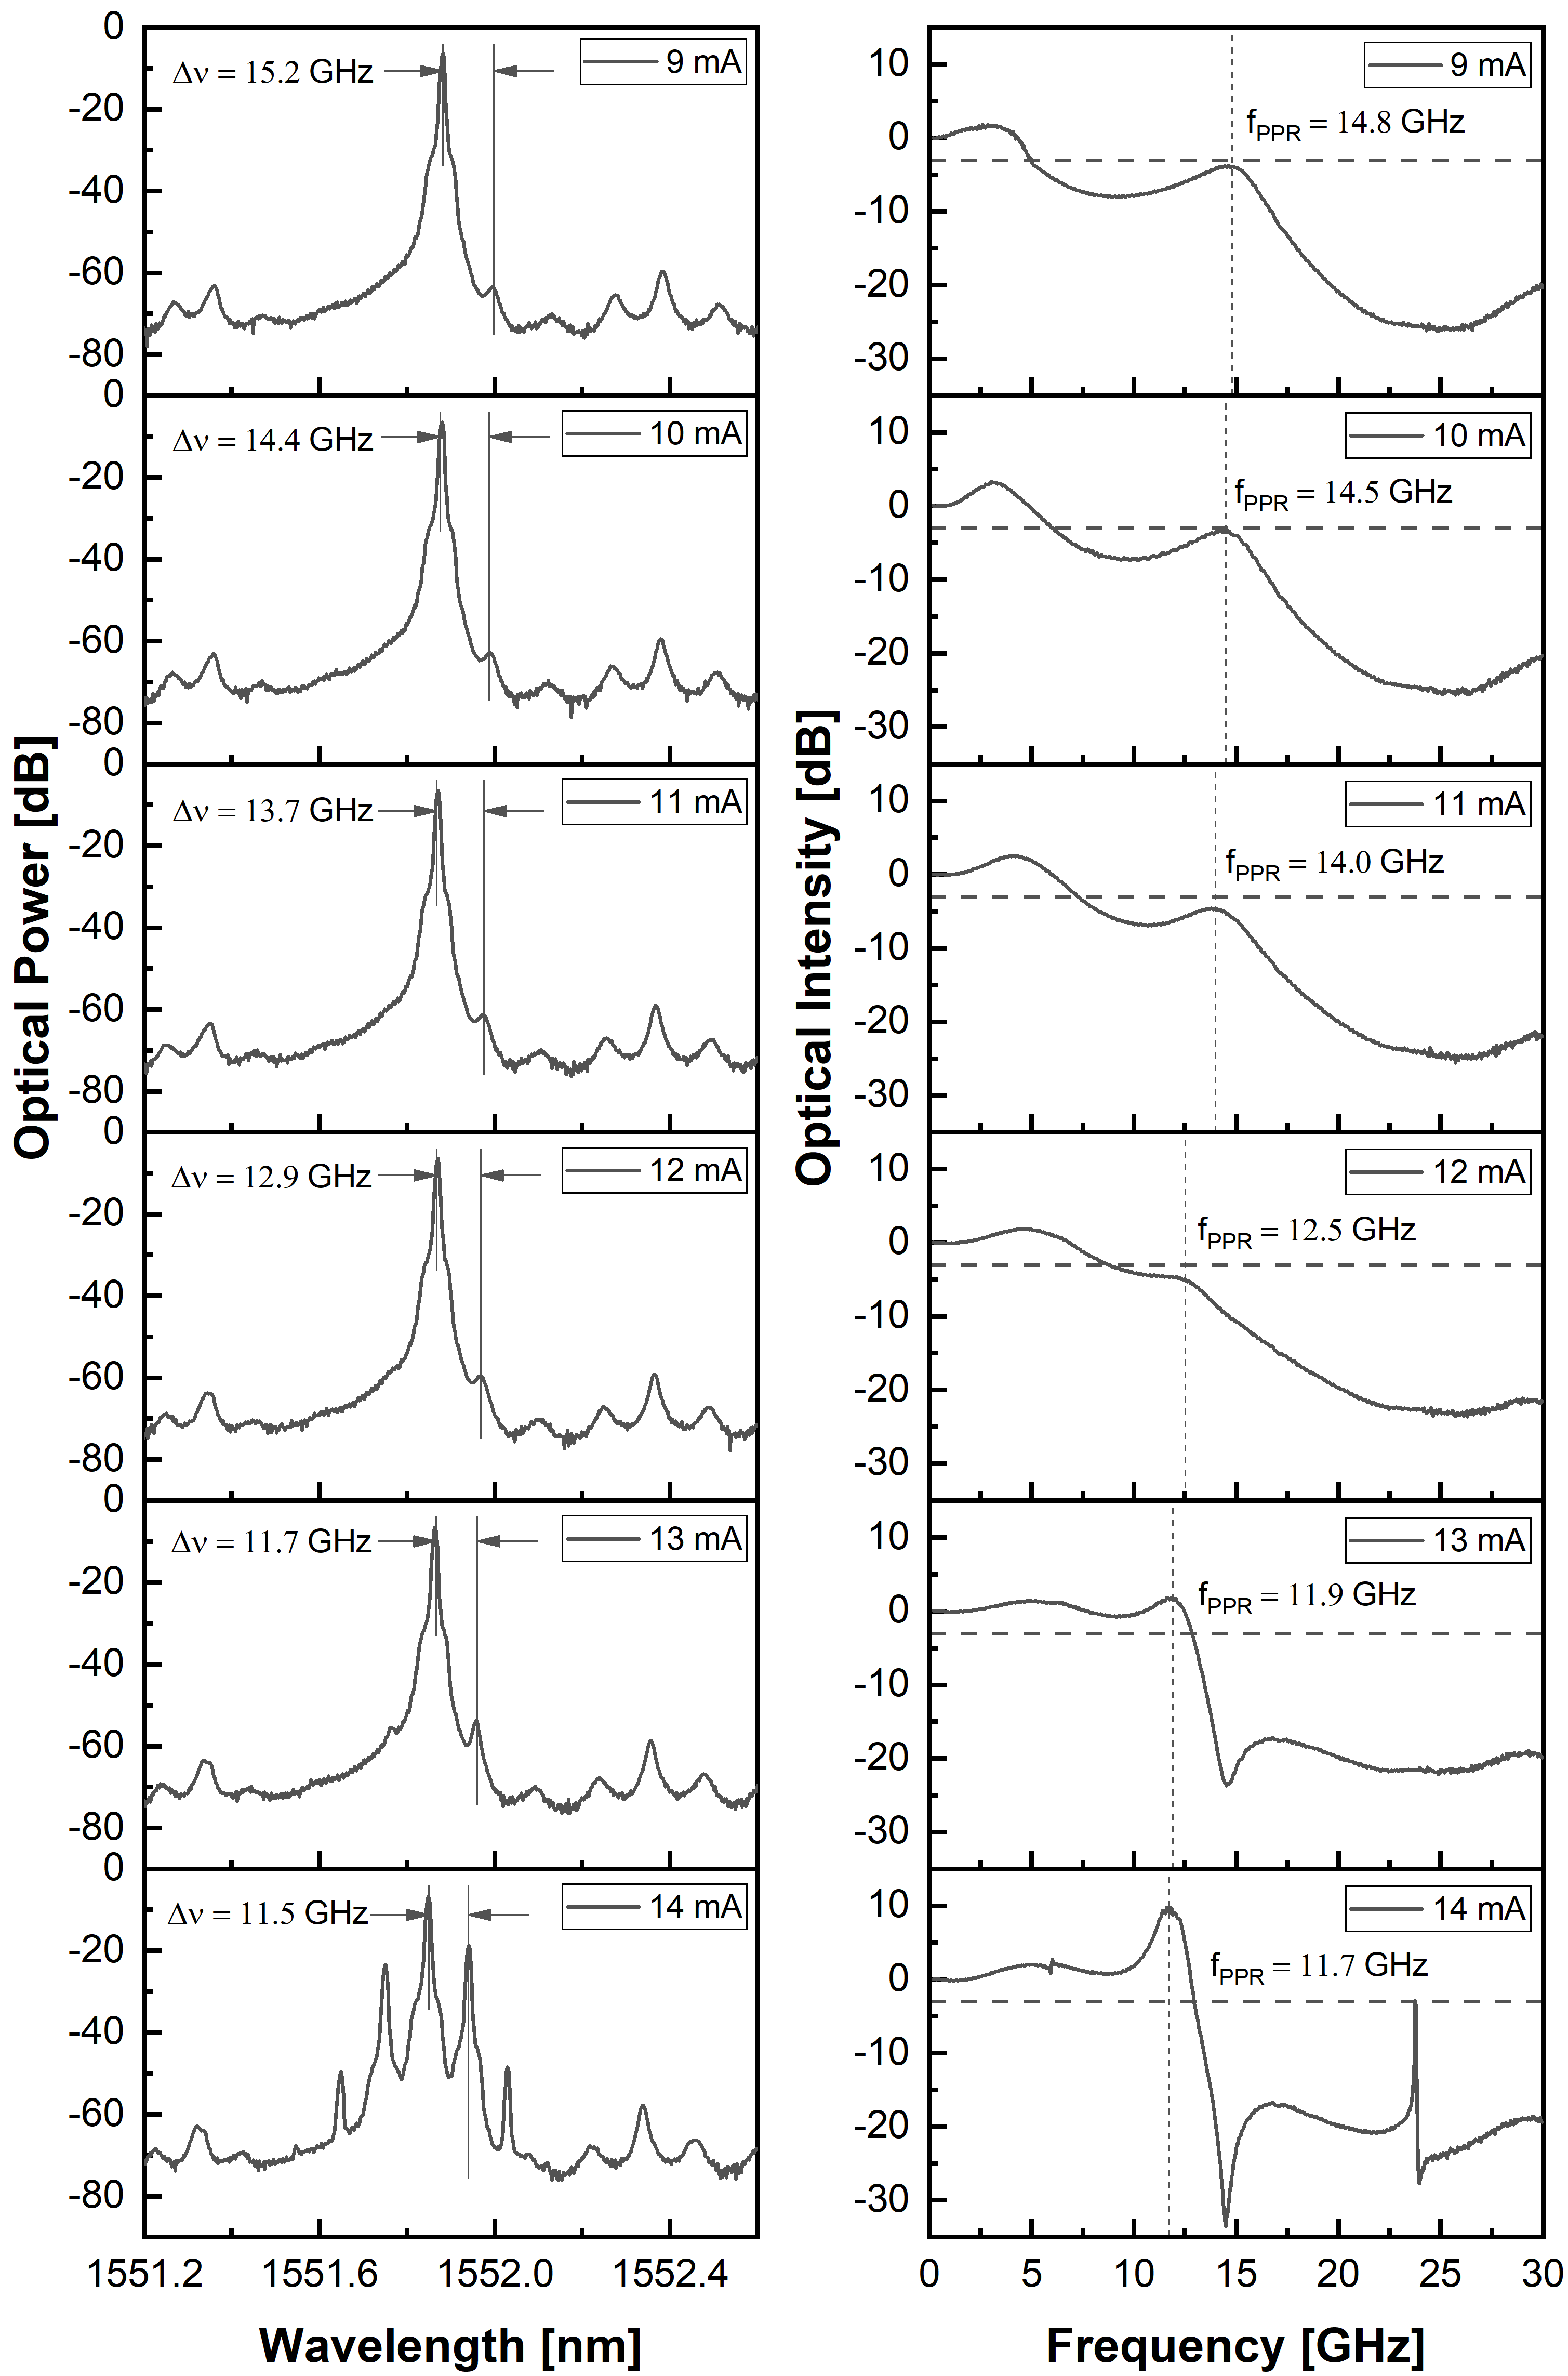
\includegraphics[width=.8\linewidth]{figures/spectra_and_bandwidth_6559.png}
    \caption{}
    \label{fig:spectra_and_bandwidth_6559}
\end{figure}

\begin{figure}[!htb]
    \centering
    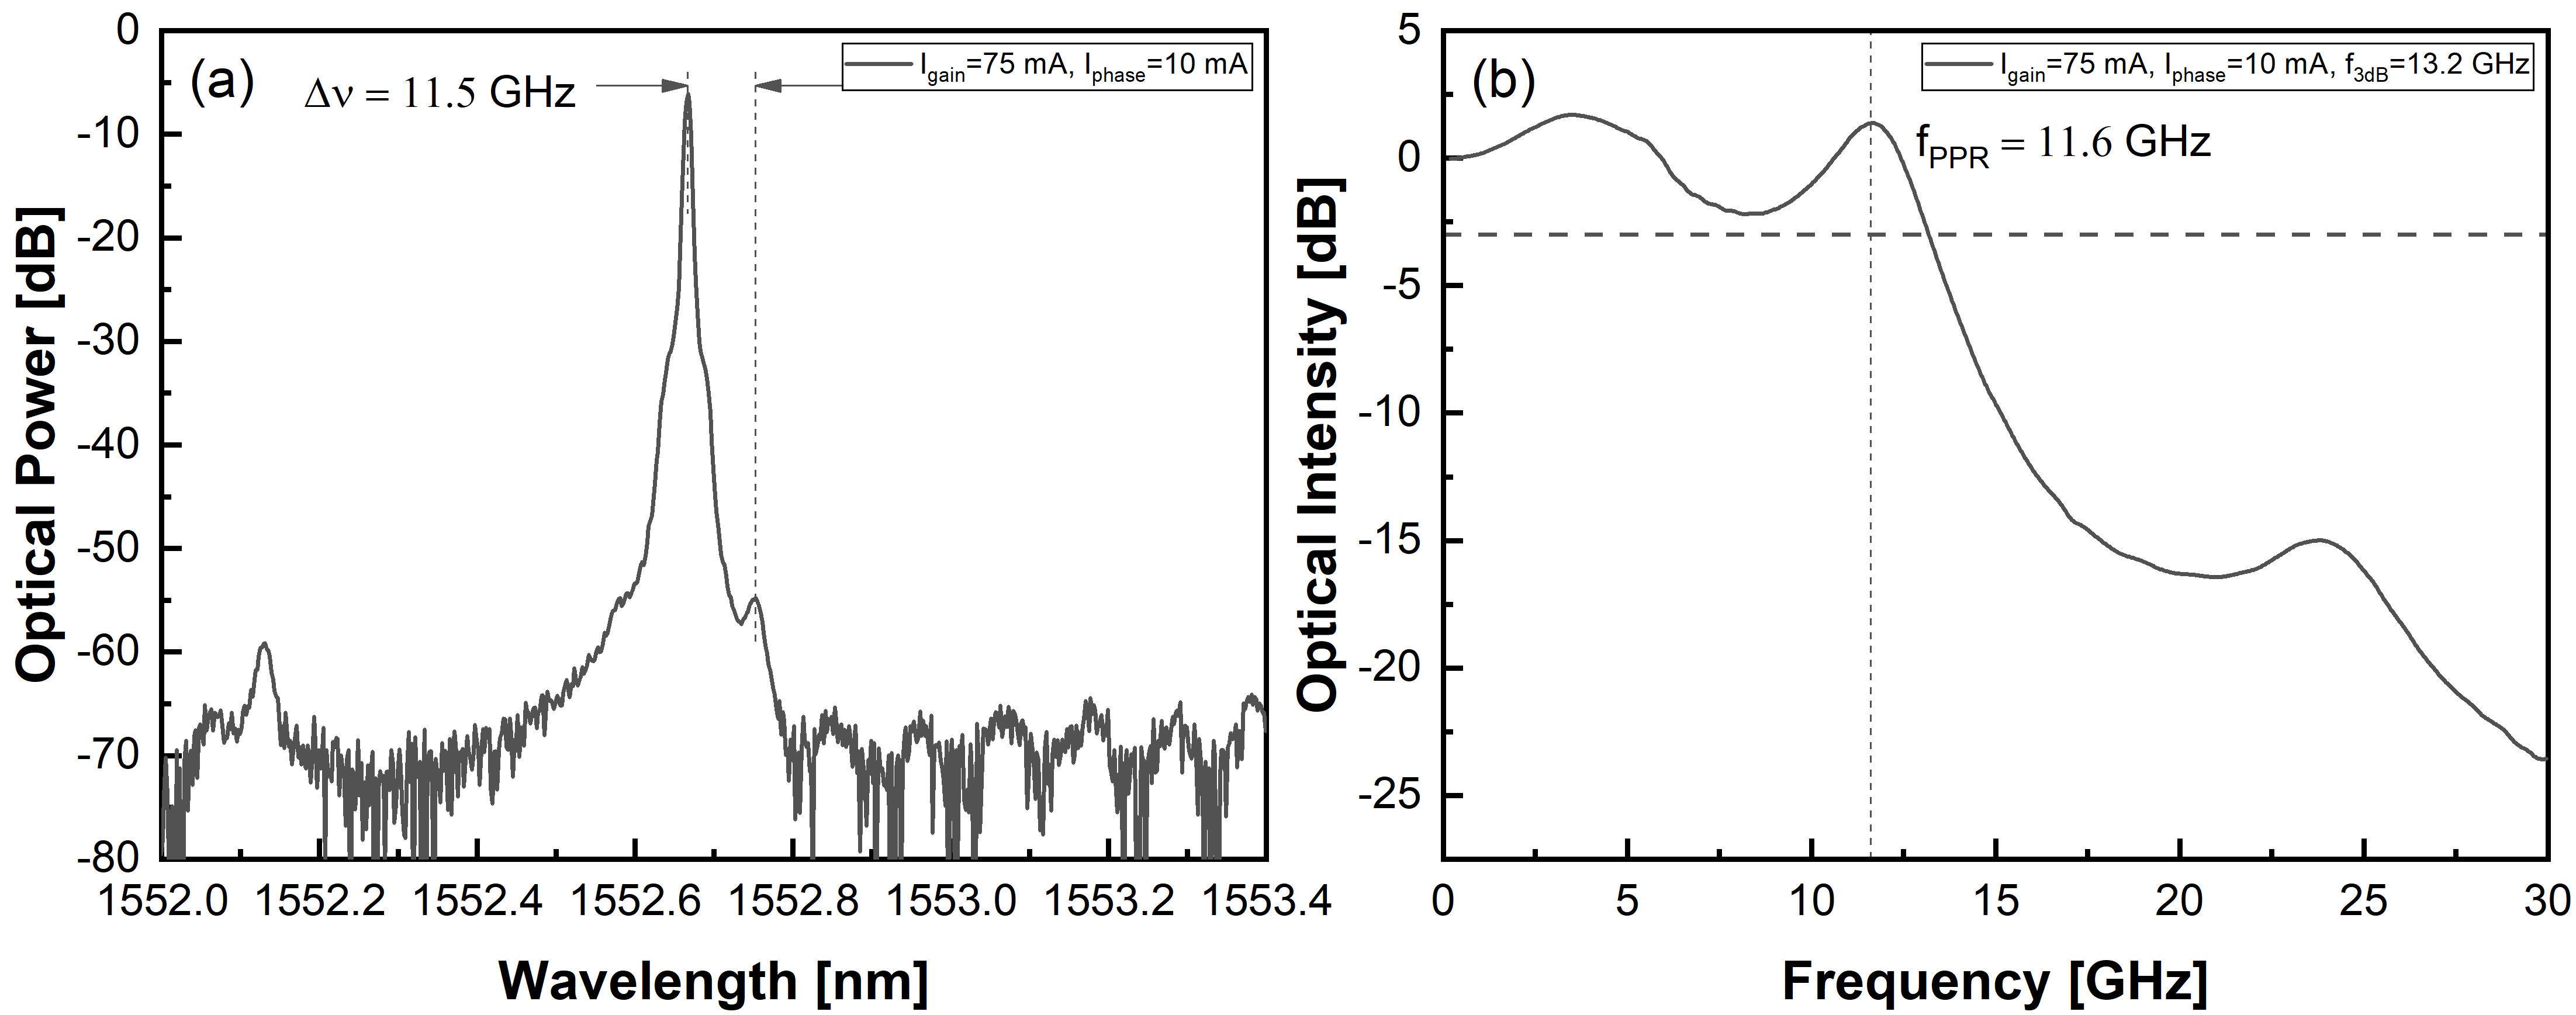
\includegraphics[width=\linewidth]{figures/spectrum_and_bandwidth_6557.png}
    \caption{}
    \label{fig:spectra_and_bandwidth_6557}
\end{figure}

\begin{figure}[!htb]
    \centering
    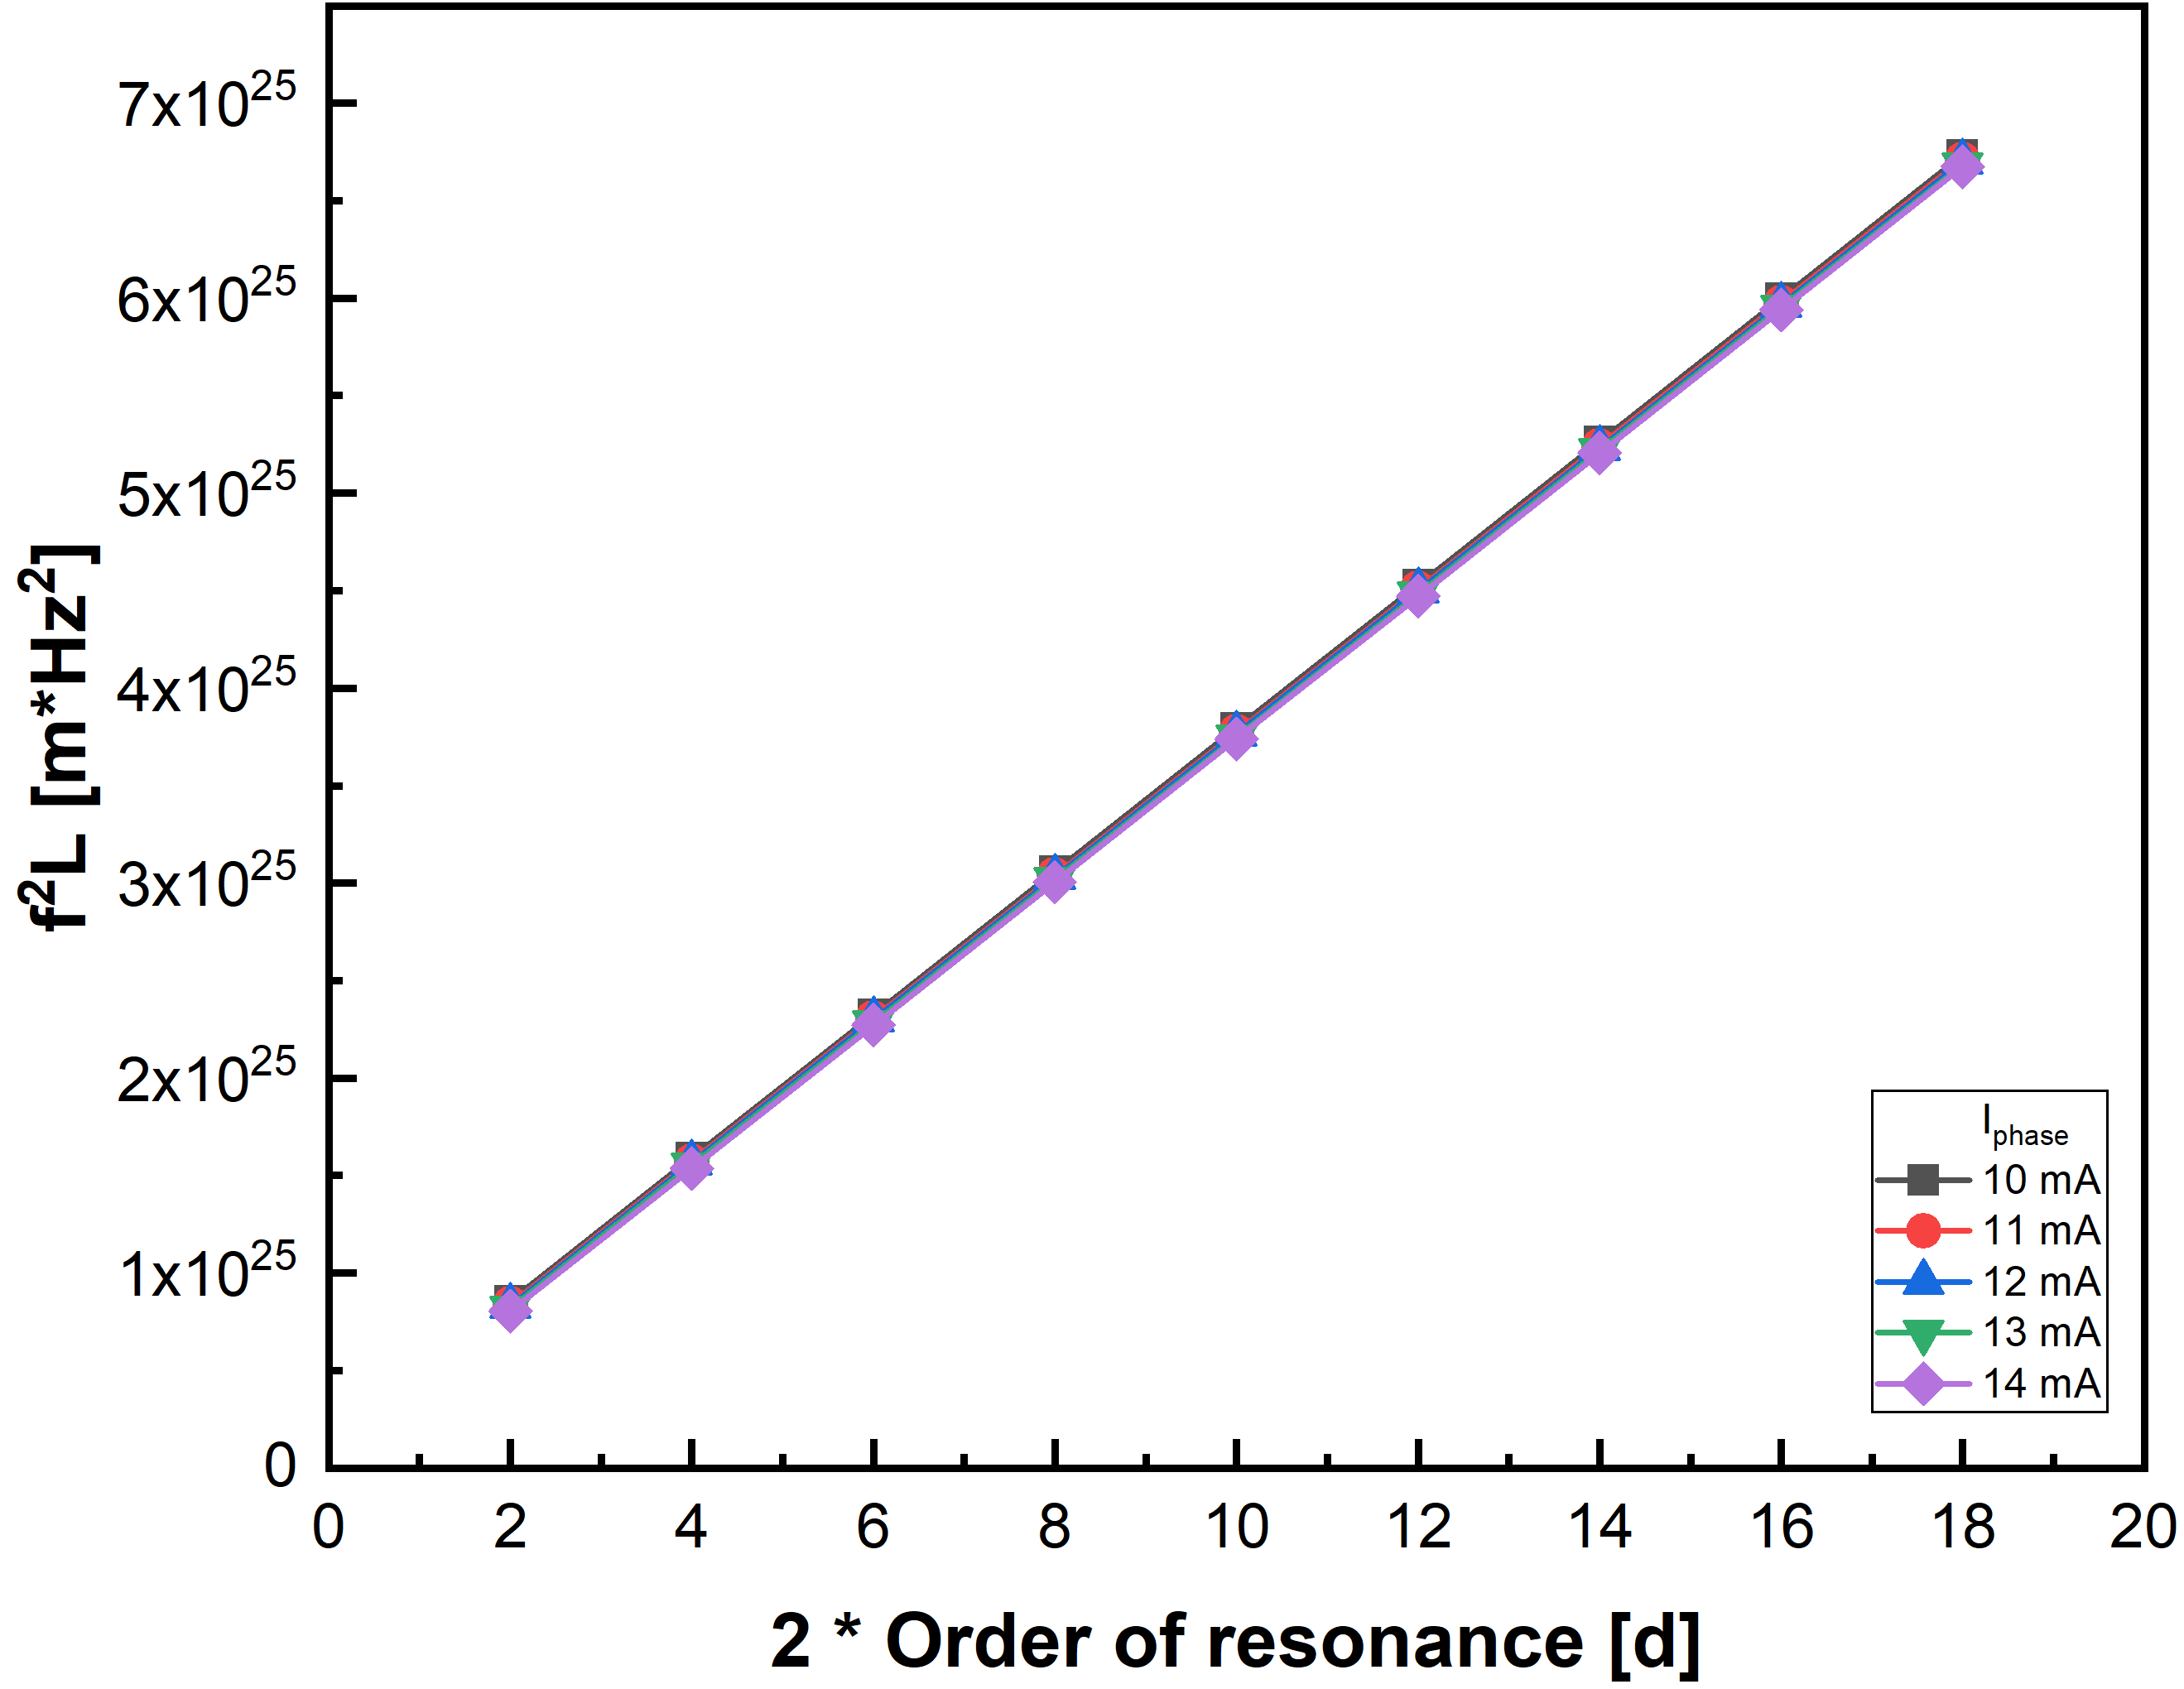
\includegraphics[width=.7\linewidth]{figures/chirp_6559.png}
    \caption{}
    \label{fig:chirp_6559}
\end{figure}

\begin{table}[!htb]
    \centering
    \caption{My caption}
    \label{my-label}
    \begin{tabular}{@{}llllll@{}}
    \toprule
    \multirow{2}{*}{Current {[}mA{]}} & \multicolumn{5}{c}{$\alpha$}                                                                                \\ \cmidrule(l){2-6} 
                                      & $I_{phase}=10 \ mA$ & $I_{phase}=11 \ mA$ & $I_{phase}=12 \ mA$ & $I_{phase}=13 \ mA$ & $I_{phase}=14 \ mA$ \\ \midrule
    75                                & 1.725               & 2.063               & 2.22                & 2.624               & 3.247               \\
    75                                & 1.818               & 1.991               & 2.296               & 2.618               & 3.257               \\
    75                                & 1.818               & 2.07                & 2.246               & 2.614               & 3.253               \\
    75                                & 1.808               & 2.054               & 2.242               & 2.566               & 3.221               \\ \midrule
    Average                           & 1.79225             & 2.0445              & 2.251               & 2.6055              & 3.2445              \\ \bottomrule
    \end{tabular}
\end{table}